\begin{frame}
    \frametitle{Feed Forward Neural Network}
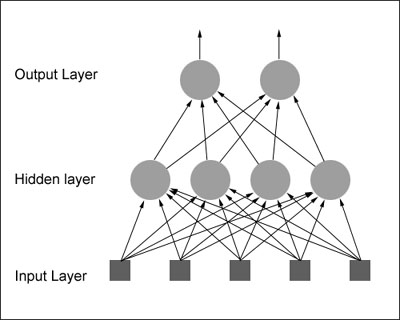
\includegraphics[width=0.7\textwidth]{simple_feedforward_network}
\end{frame}


\begin{frame}
\frametitle{State of hidden neurons}
\[
  \eta_{i} =
  \Phi \left(
    \sum_{j=1}^{n}
    w_{i,j}\,x_j + \text{bias}_{i,1}
  \right)
\]
\end{frame}

\begin{frame}
\frametitle{State of output neurons}
\[
  \gamma_{i} =
  \Phi\left(
    \sum_{j=1}^{h}
    \delta_{i,j}\,\eta_i + \text{bias}_{i,2}
  \right)
\]
\end{frame}

\begin{frame}
    \frametitle{Input-hidden weights}
  \[
    W_{h \times {n+1}} =
    \left[
      \begin{array}{ccc|c}
        w_{1, 1} & \cdots & w_{1, n} & w_{1, n+1} \\
        \vdots   & \ddots & \vdots   & \vdots     \\
        w_{h, 1} & \cdots & w_{h, n} & w_{h, n+1}
      \end{array}
    \right],
  \]
\end{frame}

\begin{frame}
    \frametitle{Hidden-output weights}
  \[
    \Delta_{m \times h+1} =
    \left[
      \begin{array}{ccc|c}
        \delta_{1,1} & \cdots & \delta_{1,h} & \delta_{1,h+1}\\
        \vdots & \ddots &  \vdots & \vdots\\
        \delta_{m,1} & \cdots & \delta_{m,h} &\delta_{m,h+1}
      \end{array}
    \right],
  \]
\end{frame}

\begin{frame}
\frametitle{Algorithm}
\begin{align}
\eta &= Wx \\
\eta &= \Phi(\eta) \\
\gamma &= \Delta\eta \\
\gamma &= \Phi(\gamma)
\end{align}
\end{frame}


\begin{frame}
\frametitle{Arquitecture of the solution}
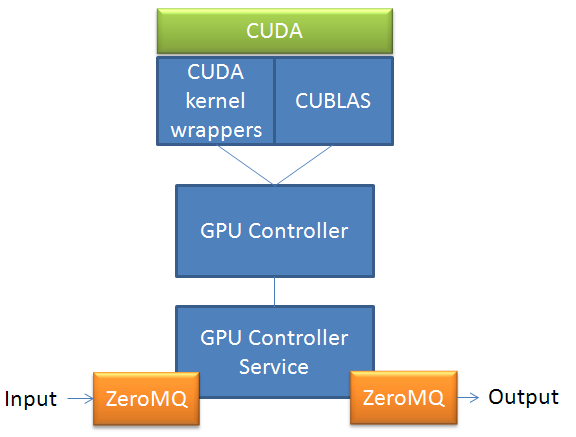
\includegraphics[width=0.7\textwidth]{arq}
\end{frame}

\begin{frame}
    \frametitle{Interaction diagram}
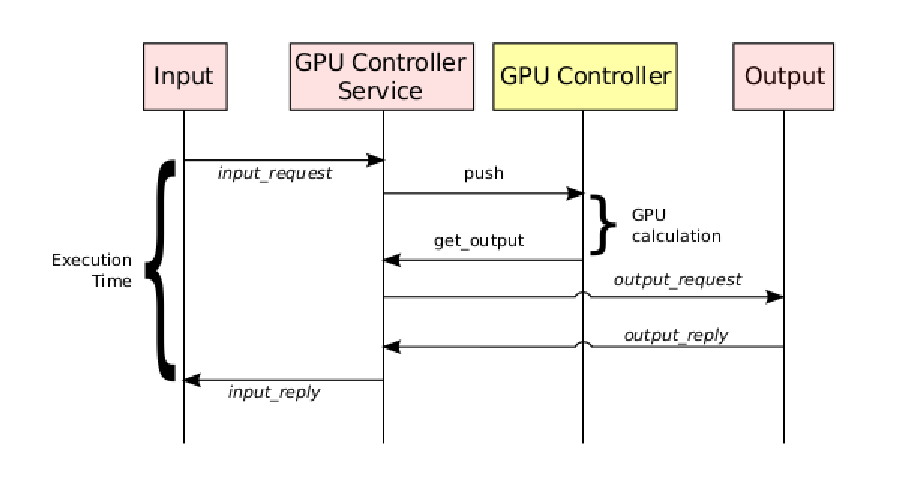
\includegraphics[width=0.7\textwidth]{../interaction-diagram-eps-converted-to.pdf}
\end{frame}



\begin{frame}
      \frametitle{CUBLAS}
      \lstinputlisting{src/cublas.cu}
\end{frame}

\begin{frame}
      \frametitle{CUDA kernels}
      \lstinputlisting[basicstyle=\small]{src/kernels.cu}
\end{frame}

\begin{frame}
      \frametitle{Results}
\begin{itemize}
\item Typical problem: \(2000\times5000\times 500\).
\item Time limit requirement: 1 millisecond.
\item Actual execution time: order of \(0.25\) milliseconds.
\item Intel Xeon CPU E5520 2.27GHz.
\item NVIDIA Tesla C1060.
\end{itemize}
\end{frame}

\begin{frame}
      \frametitle{Takeaways}
\begin{itemize}
\item Activation function time is negligible (~2\%).
\item It is not worth the effort to integrate 4 operations into one kernel.
\item Only fine tuning needed: keep occupancy high.
\item Separation into simple components makes testing easier.
\item Hard limit met easily by the GPU, not by the CPU.
\end{itemize}
\end{frame}



